\documentclass[]{article}
\usepackage{amsmath}
\usepackage{amsfonts}
\usepackage{amssymb}
\usepackage{graphicx}
\usepackage{float}
\usepackage{listings}
\usepackage{color}

\definecolor{mygreen}{rgb}{0,0.6,0}
\definecolor{mygray}{rgb}{0.5,0.5,0.5}
\definecolor{mymauve}{rgb}{0.58,0,0.82}

\lstset{ %
	backgroundcolor=\color{white},   % choose the background color
	basicstyle=\footnotesize,        % size of fonts used for the code
	breaklines=true,                 % automatic line breaking only at whitespace
	captionpos=b,                    % sets the caption-position to bottom
	commentstyle=\color{mygreen},    % comment style
	escapeinside={\%*}{*)},          % if you want to add LaTeX within your code
	keywordstyle=\color{blue},       % keyword style
	stringstyle=\color{mymauve},     % string literal style
}

\bibliography{DynamicsFinalProject}


%opening
\title{ENGR 2340 Final Project: Computational Modeling of Aerodynamic Flutter}
\author{Arpan Rau}

\begin{document}

\maketitle

\begin{abstract}

This project models Aerodynamic Flutter in a wing section. Flutter is a sometimes-divergent condition that occurs when the combination of elastic and aerodynamic forces on a wing cause oscillations.

For the purposes of this model, the following equations of motion for a wing in flutter conditions were derived:

$\ddot{\theta} = \dfrac{x_{ac} \dfrac{1}{2} \rho u^2 S C_{l\alpha} - \dfrac{l}{\theta JG}}{I_{wing}}$


$\ddot{z} = \dfrac{\dfrac{1}{2} \rho u^2 S C_{l\alpha}-\dfrac{l^3}{3zEI}}{M_{wing}}$

The model solves the differential equations above discretely in small timesteps.

The all-MDF monotonic wing section analyzed was too stiff and had a center of gravity too far forward to experience divergent flutter conditions, but the system did display oscillations, both in bending and torsion. This model, coupled with empirical airfoil lift coefficient data, could be used to predict flutter on less stiff or structurally more complex wings. 

The project's Codebase can be found at:
 https://github.com/arpanrau/aerodynamic-flutter. 




\end{abstract}

\section{Project Background}

This project's primary goal is to produce a Python Model of Aerodynamic flutter.There are many different types of airfoil flutter, but the basic 'Pitch-Plunge' mechanism, which will be the focus of this project, is such :

\begin{enumerate}
	\item Flutter is initiated by a rotation of the airfoil to a positive angle of attack
	\item As the increased aerodynamic lift causes the airfoil to rise, the torsional stiffness of the structure returns the airfoil to 0 angle of attack.
	\item The bending stiffness of the wing returns the airfoil to a neutral position, but the airfoil rotates into a negative angle of attack
	\item The aerodynamic force causes the airfoil to plunge and torsional stiffness returns the airfoil to 0 angle of attack.
	\item The bending stiffness of the wing returns the airfoil to a neutral position, but at a positive angle of attack.
\end{enumerate}

This pattern continues. Because aerodynamic forces can twist or bend the wing farther each oscillation, this flutter can lead to the wing breaking off the aircraft. The second failure of famed early Aviator Samuel Langley's prototype on the Potomac can be attributed to flutter. \cite{article}

\begin{figure}[H]
	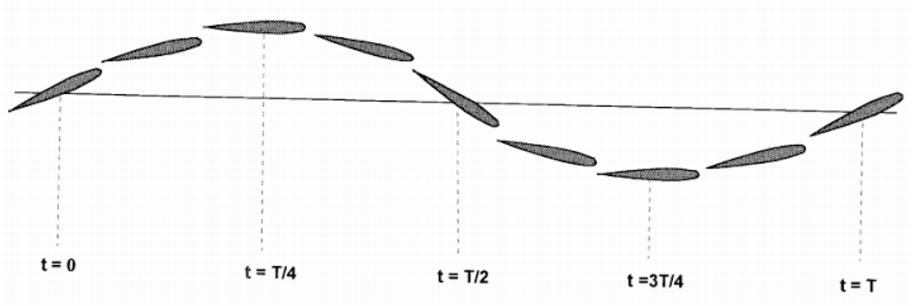
\includegraphics[width=8cm]{PitchPlunge}
	\centering
	\caption{Example of Pitch-Plunge Motion[1]}
\end{figure}


Aerodynamic flutter is a complex behavior that arises from the interplay of different forces,so it is difficult to anticipate without modeling the entire system. A flutter model must capture at a minimum aerodynamic forces, wing bending, and wing torsion, but can be expanded to include forces and moments from control surfaces, wing-mounted engine nacelles, or even fuel slosh in wing tanks (which, without baffling, can be significant). Before the causes of flutter were well-defined, Aircraft designers were forced to resort to trial and error. Nowadays, there is significant interest in better modeling flutter in wind turbines, allowing for blades that have a wider range of operating conditions. 

\section{Learning Objectives}

The primary learning goal considered in developing this project was gaining familiarity working with fluid forces and aerodynamic effects. As an Aerospace engineer, I often find myself struggling in technical interviews due to my lack of a fluids and aerodynamics background. This project was meant to bridge gaps in my interview skill-set.

In addition, I would like to refresh my working structural engineering knowledge, keeping the closed-form solutions for things like beam bending under a constant load and beam torsion in my working memory. I'd like to work with some form of web interface, as I often in industry find myself building Python models that only I am able to run. Lastly and mostly generally, I'd like to gain experience modeling dynamic systems, as opposed to the more static structures I am used to .

As such, I formulated the following goals for the project:

\begin{itemize}
	\item Produce a model which represents some form of aerodynamic instability
	\item Ensure the model provides some form of useful engineering output
	\item Produce some form of 2D GUI, Animation, or Rendering 
\end{itemize}

\section{System Model}

A pitch-plunge flutter system is a mass-spring system excited by Aerodynamic forces. Each wing section experiences Lift and Aerodynamic moments about the Aerodynamic center and an Elastic force and moment about it's Elastic axis. 
This model solves for the acceleration of the wing at each discrete time-step using $\Sigma F = MA$ and $\Sigma T = I \alpha$. It then updates wing position and velocity to reflect those values. 


\begin{figure}[H]
	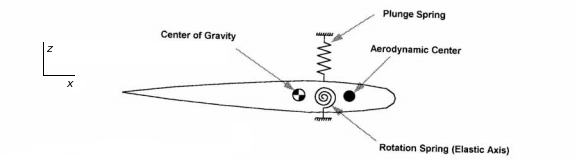
\includegraphics[width=12cm]{MassSpring}
	\centering
	\caption{Simplified System Model\cite{article}}
\end{figure}

It is important to remember that the wing is a three-dimensional structure, with each 2D wing cross-section experiencing the above effects. For modeling simplicity, this model approximates the wing as a rigid wing section of a given width attached to a massless beam section which experiences no aerodynamic effects. 


\begin{figure}[H]
	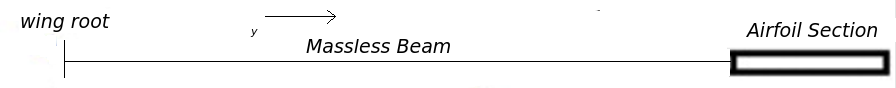
\includegraphics[width=12cm]{ds}
	\centering
	\caption{Wing planform simplification}
\end{figure}

\subsection{Driving Assumptions}

\begin{itemize}
	
	\item Wing is composed of rigid airfoil section attached to Massless Beam (Ignoring Aerodynamic forces on most of the wing to simplify model)
	
	\item Flow over the wing has a speed of less than Mach .3 (incompressible flow)
	
	\item Tip wash on wing is negligible (Airfoil can be modeled in 2D sections)
	
	\item Airfoil used is symmetric (Aerodynamic moment is 0 about Aerodynamic center)
	
	\item Flow Reynolds number is between $10^4$ and $10^7$
	
	\item Airfoil stall happens instantaneously when the airfoil passes 15 degrees angle of attack. 
	
	\item Wing is rigid in bending about z-axis (Drag can be ignored)
	
	\item Airfoil used is a NACA 16-006 airfoil of chord length .2 M , made of Medium-Density-Fiberboard
	
	\item Massless beam section was attached at center of mass of airfoil section $(X_{gc} = 0)$
	

\end{itemize}


\subsection{Symbols Used}

\begin{itemize}
	
	\item $R$ = Radius of circular beam cross-section, Meters
	\item $E$ = Modulus of Elasticity of the beam material, Pa
	\item $I$ = Moment of Inertia of the beam , Meters$^4$. For a circular beam,calculated as $\dfrac{\pi R^4}{4}$
	\item $z$ = Vertical Deflection of elastic axis, Meters
	\item $F_e$ = Elastic force due to deflection of beam, Newtons
	\item $l$ = Length of massless beam section, Meters
	\item $\theta$= Angle of wing twist about elastic axis, Radians
	\item $T_e$ = Moment exerted by beam about elastic axis, Newton*Meters
	\item $J$ = Torsional Constant of the Beam. For a circular beam, calculated as $\dfrac{\pi R^2}{2}$
	\item $G$ = Shear Modulus of Beam Material, Pa
	\item $x_{ac}$ = Distance in meters from Elastic axis to Aerodynamic Center. For this model, it is assumed both lie on the X=0 axis.
	\item $x_{fc}$ = Distance in meters from Elastic axis to Center of Gravity. For this model, it is assumed this distance is 0.
	\item$C_{l\alpha}$ = Section Lift Coefficient of Airfoil for a given angle of attack
	\item$S$ = Length of rigid airfoil section, Meters
	\item$F_l$ = Lift force generated by wing, Newtons
	\item$Rho$ = Density of Airflow over wing, kg/m$^3$
	\item$u$ = Velocity of Airflow over wing, m/s
	\item$I_{wing}$ = Moment of inertia of the airfoil section about the elastic center, Meters$^4$. Computed by modeling wing in Onshape.
	\item$M_{wing}$ = Mass of the airfoil section, Kg. Computed by modeling wing in Onshape.
	\item$\rho_{airfoil}$ = Density of airfoil, kg/m$^3$
	
	
\end{itemize}

\subsection{Elastic (Bending) Forces and Moments}

As the airfoil section of the wing is modeled as rigid, the beam section is the source of all bending forces. 

The beam section of the wing is attached to the aircraft on one end and unsupported on the other, experiencing the load of the airfoil. As such, the deflection of the beam for a given force  can be given by $z = \dfrac{-{F_e} l^3}{3EI}$.\cite{machinerys} Rearranging this in terms of $F_e$ results in $F_e = \dfrac{ -3zEI}{l^3}$

The beam acts as a torsion spring. The angular deflection (setting positive rotation to be counterclockwise rotation about the Y-Axis) about the elastic axis, $\theta = \dfrac{- T_e l}{JG}$. \cite{machinerys} Rearranging this for $T_e$ results in $T_e = \dfrac{-\theta JG}{l}$


\subsection{Aerodynamic Forces and Moments}

Because the airfoil used is symmetric, it experiences no moments about its aerodynamic center (Assumed to be located at the 1/4-chord location), and a lift force at this center. That lift force can be defined by $F_l = \dfrac{1}{2} \rho u^2 S C_{l\alpha}$  \cite{article}

$C_{l\alpha}$ for a thin symmetric airfoil can be found by thin-airfoil theory to be $C_{l\alpha} = 2 \pi \alpha $.  \cite{article} This holds true up to angles of attack of roughly 15 degrees, after which point it is assumed the wing stalls and produces no lift.

Because the aerodynamic center of the wing is not the elastic axis, the moment about the elastic axis due to the lift force is $T_l = x_{ac} F_l$. \cite{article}


\subsection{Equations of Motion}

 $\Sigma F = MA$ and $\Sigma T = I \alpha$.
 Therefore, $\alpha = \ddot{\theta} = \dfrac{\Sigma T}{I_{wing}} = \dfrac{T_e+T_l}{I_{wing}} = \dfrac{x_{ac} \dfrac{1}{2} \rho u^2 S C_{l\alpha} - \dfrac{l}{\theta JG}}{I_{wing}}$
 Similarly, $A = \ddot{z} = \dfrac{\Sigma F }{M_{wing}} = \dfrac{F_e+F_l}{M_{wing}} = \dfrac{\dfrac{1}{2} \rho u^2 S C_{l\alpha}-\dfrac{l^3}{3zEI}}{M_{wing}}$
 
 

\section{Results}

This model captures high-frequency aerodynamic flutter particularly well. Though the wing modeled does not produce divergent conditions and torsional wing failure, other wings with lower stiffnesses and more gradual stall conditions could. I think to completely capture divergent flutter phenomena, this model would have to be based off of empirical lift data (I could not find a good source for this), or 

Over the course of this project, I became far more familiar with various models of aerodynamic lift and how and where they fail.  I refreshed my structural engineering knowledge and added some closed-form solutions for beam torsion to my working knowledge. I also discovered the Jupyter-Notebook interface for Python, which allows me to write python in a browser and web-based interface and generate outputs that will display properly when pushed directly to git, satisfying my GUI learning goal. I intend to start using notebooks for my Python models in industry. 

\subsection{Visualization - Theta and Z vs Time}


\begin{figure}[H]
	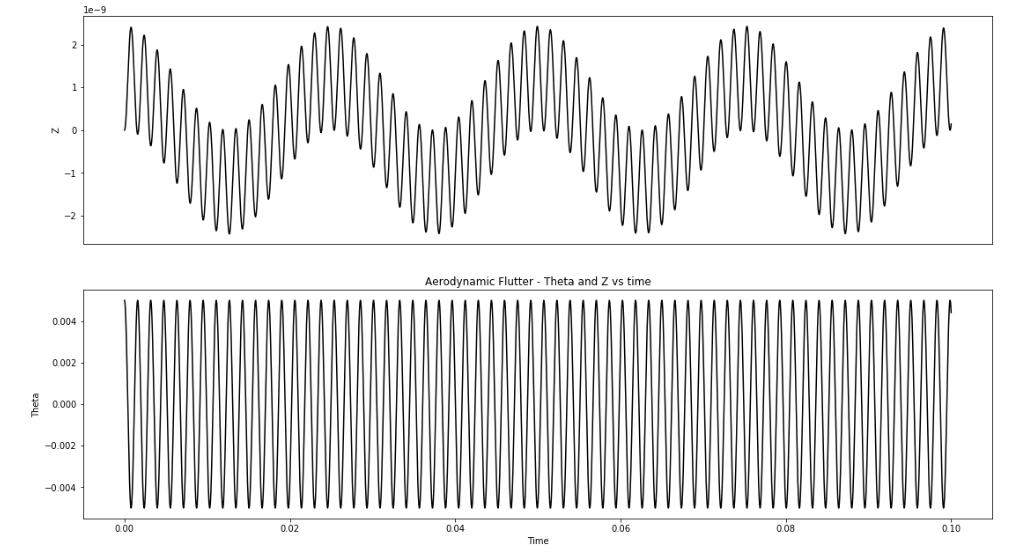
\includegraphics[width=12cm]{flutterplot}
	\centering
	\caption{Theta and Z vs time}
\end{figure}

This visualization shows theta and Z for the end of the wing vs time. It is notable that the model managed to capture two separate modes for Z vs time, one driven by wing lift changing with wing twist and the other driven by the mass and momentum of the wing itself.

This wing would be safe from dangerous flutter conditions as the wing is stiff enough that the oscillations observed are quite small. 

\section{Appendix- Code}

\begin{lstlisting}[language=python]
import numpy as np
from __future__ import division
import matplotlib.pyplot as plt


class Airfoil:
"""Model of Airfoil under Aerodynamic Flutter"""
	def __init__(self):
	
	self.runtime = .1 #how long the model will run for
	self.timestep = .00001 #Discrete timestep to run the program
	
	#constants and wing properties
	self.R = .005 #Radius of Beam Cross Section, M
	self.E = 4000000000 #Modulus of Elasticity of Beam, Pa. MDF
	self.I = 3.1415*self.R**2/4 #Moment of inertia of beam, M^4
	self.l = .8 #Length of massless beam section, Meters
	self.J = 3.1415*self.R**2/2 #Torsional constant of beam
	self.G = 2500000000 #Shear modulus of beam, PA. MDF.
	self.x_ac = .05 #distance from elastic cente to aerodynamic center,m
	self.x_gc = 0 #distance from cm of wing to aerodyanmic center, m
	self.Rho = 1.225 #density of airflow over wing, kg/m^3
	self.u = 6 #velocity of airflow over wing, m/s
	self.S = .2 #length of rigid airfoil section
	self.M_wing = 7.3 # mass of wing, Kg
	self.I_wing = .0078125 #moment of inertia of wing about elastic axis,kg*m^2
	
	#Initial values for theta and Z
	self.Theta = .005
	self.Thetadot = 0
	self.Thetadoubledot = 0
	
	self.Z = 0
	self.Zdot = 0
	self.Zdoubledot = 0
	
	
	self.run()
	
	def calculate_C_l(self):
		#if the angle of attack is greater than 15 degrees, stalled
		if np.absolute(self.Theta) > .261799:
		self.C_l = 0
		else:
		self.C_l = 2*3.141592*self.Theta
	
	def calculate_T_e(self):
		self.T_e = -(self.Theta*self.J*self.G)/self.l
	
	def calculate_F_e(self):
		self.F_e = -(3*self.Z*self.E*self.I)/self.l**3
	
	def calculate_F_l(self):
		self.F_l = .5*self.Rho*self.u**2*self.S*self.C_l
	
	def calculate_T_l(self):
		self.T_l = self.x_ac*self.F_l
	
	def run(self):
	
	
		#create arrays to track quantities of interest
		self.times = np.arange(0,self.runtime,self.timestep)
		self.stepcount = self.times.size
		self.thetas = np.zeros(int(self.stepcount))
		self.thetadots = np.zeros(int(self.stepcount))
		self.thetadoubledots = np.zeros(int(self.stepcount))
		self.zs = np.zeros(int(self.stepcount))
		self.zdots = np.zeros(int(self.stepcount))
		self.zdoubledots = np.zeros(int(self.stepcount))
		self.cls = np.zeros(int(self.stepcount))
		self.tes = np.zeros(int(self.stepcount))
		self.fes = np.zeros(int(self.stepcount))
		self.tls = np.zeros(int(self.stepcount))
		self.fls = np.zeros(int(self.stepcount))
		
		
		#track what step we are in
		self.step=0
		
		for t in self.times:
			#calculate quantities of interest
			self.calculate_C_l()
			self.calculate_T_e()
			self.calculate_F_e()
			self.calculate_F_l()
			self.calculate_T_l()
			
			#Calculate accelerations based on positions
			self.Thetadoubledot = (self.T_e + self.T_l)/self.I_wing
			self.Zdoubledot = (self.F_e + self.F_l)/self.M_wing
			
			#Write arrays
			self.thetas[self.step] = self.Theta
			self.thetadots[self.step] = self.Thetadot
			self.thetadoubledots[self.step] = self.Thetadoubledot
			self.zs[self.step] = self.Z
			self.zdots[self.step] = self.Zdot
			self.zdoubledots[self.step] = self.Zdoubledot
			self.cls[self.step] = self.C_l
			self.tes[self.step] = self.T_e
			self.fes[self.step] = self.F_e
			self.tls[self.step] = self.T_l
			self.fls[self.step] = self.F_l
			
			#update velocities
			self.Thetadot += self.Thetadoubledot*self.timestep
			self.Zdot += self.Zdoubledot*self.timestep
			
			#update positions
			self.Z += self.Zdot*self.timestep
			self.Theta += self.Thetadot*self.timestep
			
			#iterate step counter
			self.step+= 1
		
		#Plot results
		fig, ax = plt.subplots(2)
		
		plt.title("Aerodynamic Flutter - Theta and Z vs time")
		
		ax[0].plot(self.times, self.zs, 'k', label='Z')
		ax[1].plot(self.times, self.thetas ,'k', label='Theta')
		
		
		ax[1].set_xlabel("Time")
		
		ax[0].set_ylabel("Z")
		ax[1].set_ylabel("Theta")
		
		
		ax[0].axes.get_xaxis().set_visible(False)
		
		
		fig.set_size_inches(18.5,10.5)
		plt.show()

\end{lstlisting}

\begin{thebibliography}{9}

	
	\bibitem{machinerys} 
	Oberg, E. and McCauley,C.J.(2012)
	\textit{Machinery's handbook: A reference book for the mechanical engineer, designer, manufacturing engineer, draftsman, toolmaker, and machinist}.
	New York: Industrial Press
	
	\bibitem{article} 
	Hebert,Cowan, et al : Aerodynamic Flutter
	\\\texttt{http://dl.btc.pl/kamami\textunderscore wa/hk\textunderscore24474\textunderscore2.pdf}
\end{thebibliography}

\end{document}
